\documentclass{article}
\usepackage[utf8]{inputenc}
\usepackage{amsmath}
\usepackage{amssymb}
\usepackage{amsthm}
\usepackage{cancel}
\usepackage[shortlabels]{enumitem}
\usepackage{caption}
\usepackage{graphicx}
\usepackage[top=0.5in, bottom=0.5in, left=1in, right=1in]{geometry}
\usepackage{float}

% \usepackage{titlesec}
%     \titlespacing{\subsection}{\parindent}{15pt}{12pt}

\title{\textbf{\underline{CSCI4150U: Data Mining}\\Lab 04}}
\author{Syed Naqvi\\100590852}
\date{\today}

\begin{document}

    \maketitle

    \section*{Preprocessing}
    \subsection*{German Credit Data (K-NN)}
    
    This dataset contains a mixture of ordinal, nominal and numeric features. The ordinal and nominal
    features must be processed such that Minkowski distance provides a meaningful metric
    during k nearest neighbors classifications while retaining as much information as possible.
    We begin with the following features which have either a completely arbitrary ordering or
    contain only 2 unique values:

    \begin{itemize}
        \item attribute 4: Purpose
        \begin{itemize}
            \item a list of purchases on credit
        \end{itemize}
        \item attribute 9: Personal status and sex
        \begin{itemize}
            \item an arbitrarily ordered list of marital status and sex
        \end{itemize}
        \item attribute 19: Telephone
        \begin{itemize}
            \item either have a Telephone (yes) or do not (no)
        \end{itemize}
        \item attribute 20: Foreign worker
        \begin{itemize}
            \item either is a foreign worker (yes) or is not (no)
        \end{itemize}
    \end{itemize}
    
    \newpage

    We can use \textbf{one-hot encoding} for Attributes 4 and 9 as these features have multiple
    unique values and \textbf{label encoding} for attributes 19 and 20 as these features have
    only two unique values which makes ordering of label encoding irrelevant.

    \begin{figure}[H]
        \centering
        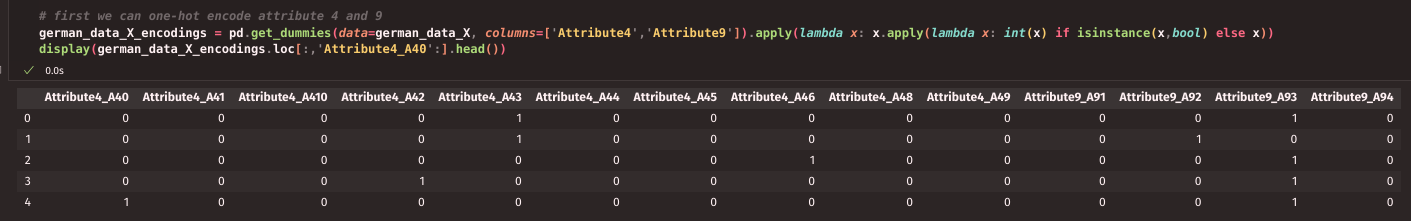
\includegraphics[width=\textwidth, height=0.13\textheight]{./I_1_g_a.png}
        \caption{[Attributes 4 and 9 one-hot encoding]}
    \end{figure}
    \begin{figure}[H]
        \centering
        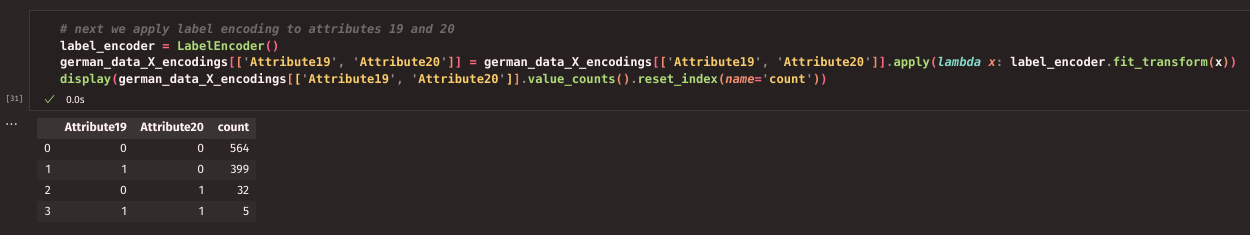
\includegraphics[width=\textwidth, height=0.13\textheight]{./I_1_g_b.png}
        \caption{[Attributes 19 and 20 label encoding]}
    \end{figure}

    The next set of features appear to have a clear ordinal ranking based on descriptions provided at (https://archive.ics.uci.edu/dataset/144/statlog+german+credit+data)
    with least credit-worthy values on the left to most credit-worthy values on the right:
    \begin{itemize}
        \item Attribute 1: Status of existing checking account
        \begin{itemize}
            \item A11 ($<$ 0 DM) $\to$ A12 (0 $<=$ \& $<$ 200 DM) $\to$ A13 ($>=$ 200 DM / salary assignments for at least 1 year) $\to$ A14 (no checking account)
        \end{itemize}
        \item Attribute 3: Credit history
        \begin{itemize}
            \item A34 (critical account / other credits existing) $\to$ A33 (delay in paying off in the past) $\to$ A32 (existing credits paid back duly till now) $\to$ A31 (all credits at this bank paid back duly) $\to$ A30 (no credits taken / all credits paid back duly)
        \end{itemize}
        \item Attribute 6: Savings account / bonds
        \begin{itemize}
            \item A61 ($<$ 100 DM) $\to$ A62 (100 $<=$ \& $<$ 500 DM) $\to$ A63 (500 $<=$ \& $<$ 1000 DM) $\to$ A64 ($>=$ 1000 DM) $\to$ A65 (unknown / no savings account)
        \end{itemize}
        \item Attribute 7: Present employment since
        \begin{itemize}
            \item A71 (unemployed) $\to$ A72 ($<$ 1 year) $\to$ A73 (1 $<=$ \& $<$ 4 years) $\to$ A74 (4 $<=$ \& $<$ 7 years) $\to$ A75 ($>=$ 7 years)
        \end{itemize}
        \item Attribute 12: Property
        \begin{itemize}
            \item A124 (unknown / no property) $\to$ A123 (car or other, not in attribute 6) $\to$ A122 (building society savings agreement / life insurance) $\to$ A121 (real estate)
        \end{itemize}
        \item Attribute 17: Job
        \begin{itemize}
            \item A171 (unemployed / unskilled - non-resident) $\to$ A172 (unskilled - resident) $\to$ A173 (skilled employee / official) $\to$ A174 (management / self-employed / highly qualified employee / officer)
        \end{itemize}
    \end{itemize}

    \newpage

    We can visualize the value distributions of each feature for each class:

    \begin{figure}[H]
        \centering
        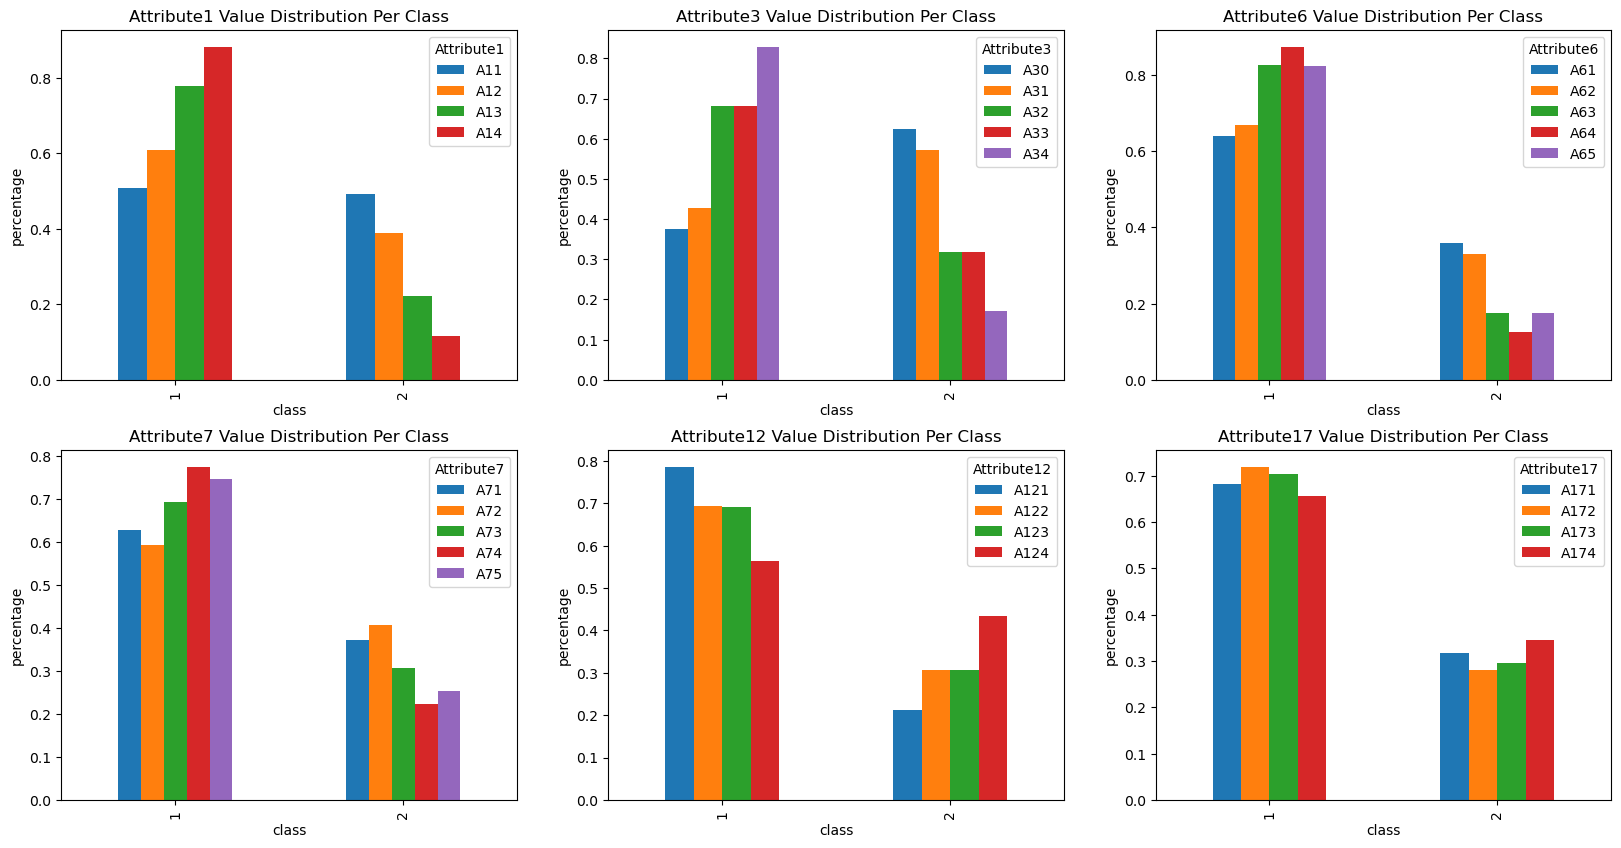
\includegraphics[width=\textwidth, height=0.3\textheight]{./I_1_g_c.png}
        \caption{[Ordinal Features Visualization (Original Labeling)]}
    \end{figure}

    It can clearly be observed that the features do seem to closely adhere to their listed orderings and for features that do not, we can re-label them so their
    lexicographical order better fits the feature's observed order. This results in the following updated class distributions:

    \begin{figure}[H]
        \centering
        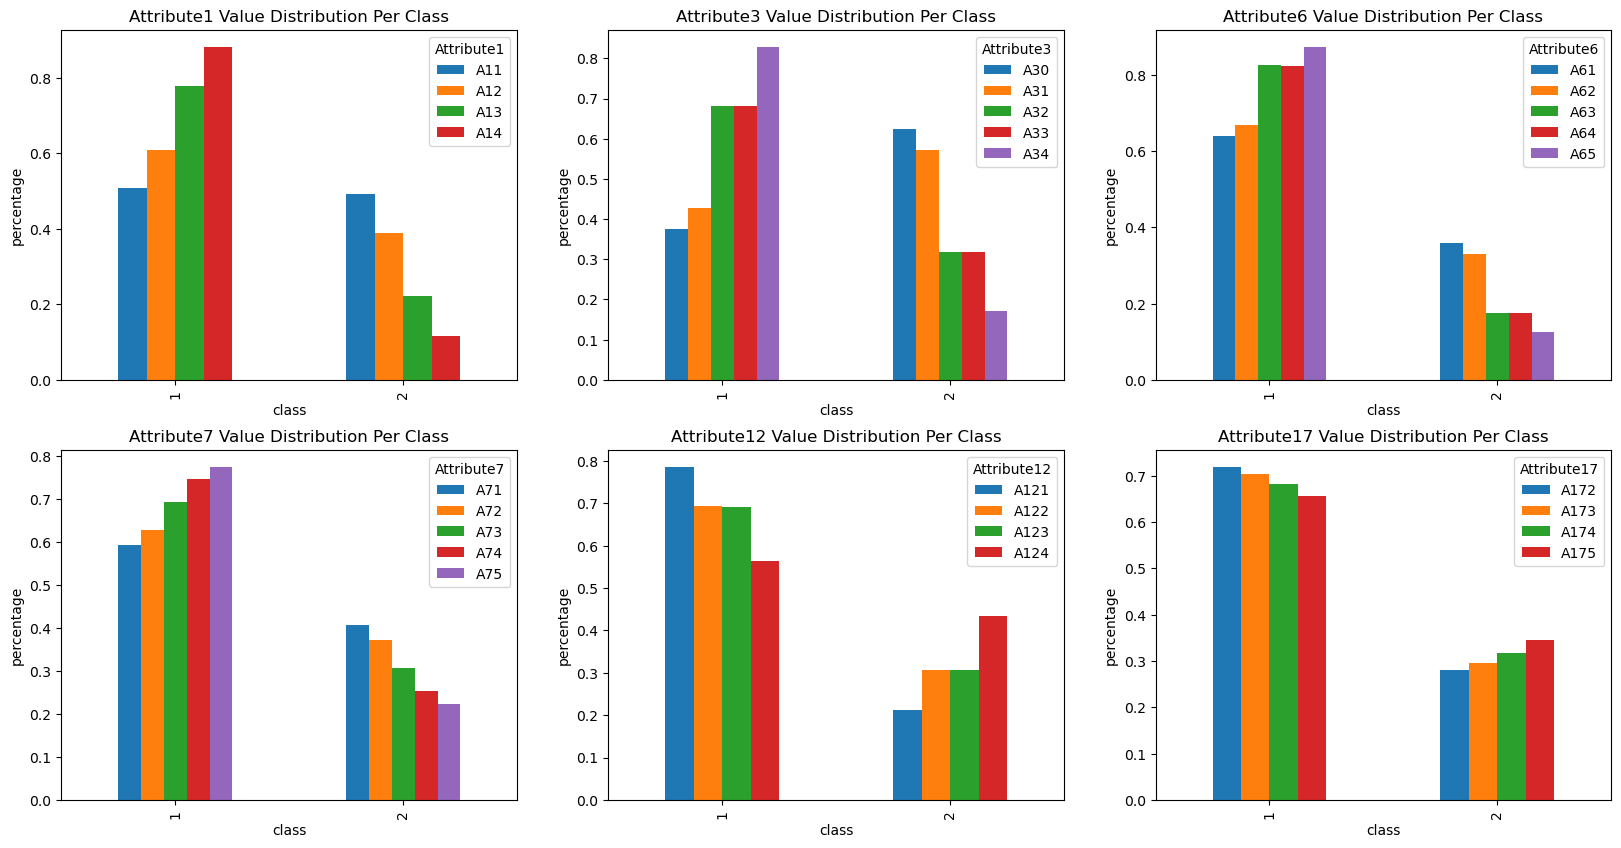
\includegraphics[width=\textwidth, height=0.3\textheight]{./I_1_g_d.png}
        \caption{[Ordinal Features Visualization (Re-Labelled)]}
    \end{figure}
    
    \newpage

    Label encoding the above features should now result in labels that better capture feature order, allowing for more meaningful distance measures between objects
    during k-nearest neighbors classification.
    \begin{figure}[H]
        \centering
        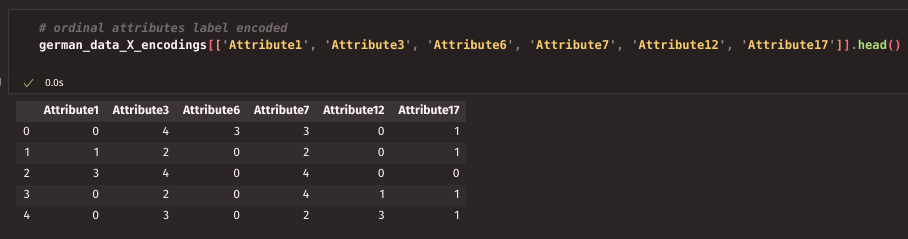
\includegraphics[width=\textwidth, height=0.15\textheight]{./I_1_g_e.png}
        \caption{[Ordinal Features Visualization (Re-Labelled)]}
    \end{figure}



    For the remaining qualitative features, we can use a similar plotting method as above to explore the existence of order.
    Based on the strength of potential orderings, we can either re-label values and then proceed with label encoding or apply one-hot encoding.

    \begin{figure}[H]
        \centering
        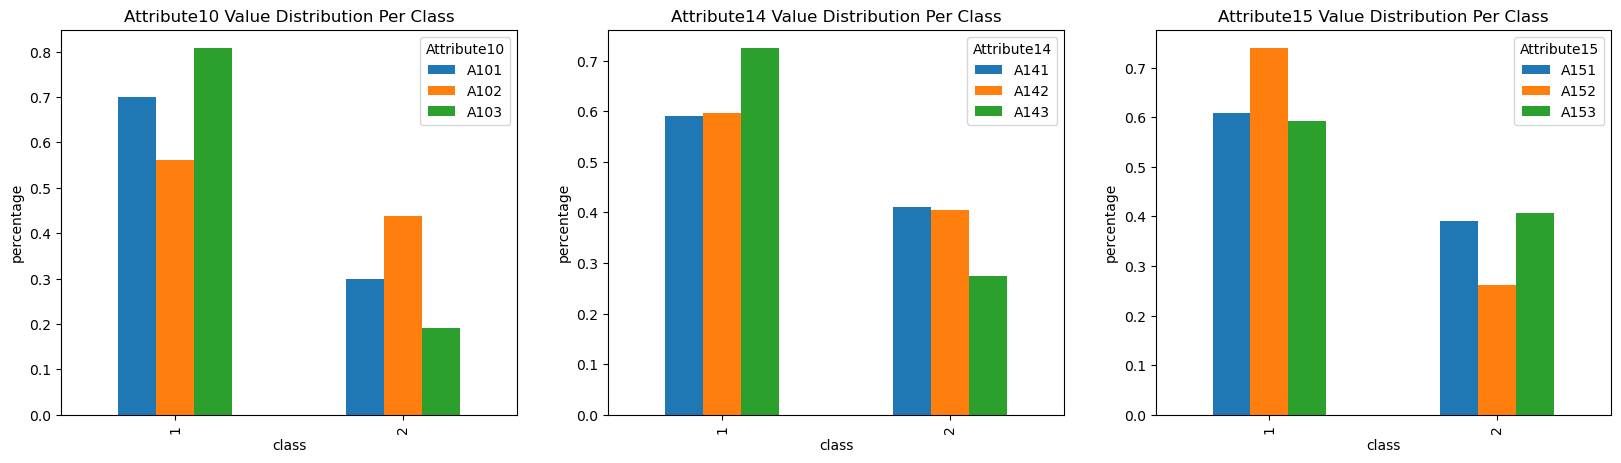
\includegraphics[width=\textwidth, height=0.2\textheight]{./I_1_g_f.png}
        \caption{[Qualitative Features Visualization (Original Labeling)]}
    \end{figure}
    
    Only Attribute 10 seems to contain a useful order relation from least credit-worthy to most credit-worthy as follows:
    \begin{itemize}
        \item A102 (co-applicant) $\to$ A101 (no debtors/guarantors) $\to$ A103 (guarantor) 
    \end{itemize}
    Attributes 14 and 15 do not seem to possess meaningful orderings as 2 out of 3 values for both features have an almost equal distribution across both classes.
    Hence, we shall re-label Attribute 10 to change its lexicographical order before applying label encoding and apply one-hot encoding to Attributes 14 and 15.
    \begin{figure}[H]
        \centering
        \begin{minipage}[t]{0.35\textwidth}
            \centering
            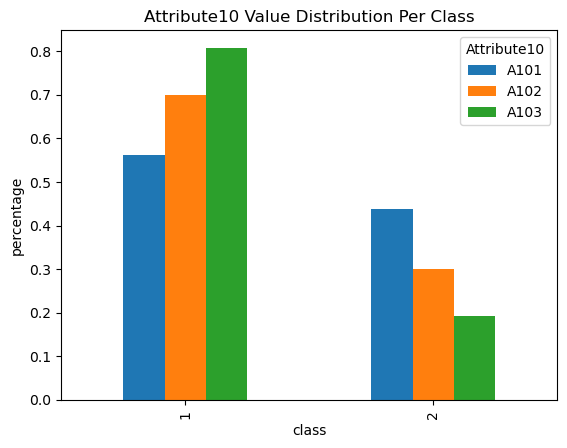
\includegraphics[width=\textwidth, height=0.2\textheight]{./I_1_g_g.png}
            \caption{[Attribute 10 Visualization (Re-Labeled)]}
        \end{minipage}
        \hfill
        \begin{minipage}[t]{0.62\textwidth}
            \centering
            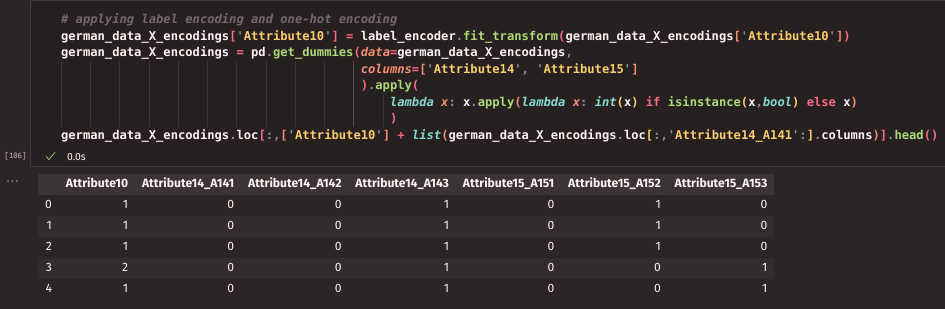
\includegraphics[width=\textwidth, height=0.15\textheight]{./I_1_g_h.png}
            \caption{[Attribute 10 Label Encoding, Attributes 14 \& 15 One-Hot Encoding]}
        \end{minipage}
    \end{figure}

    \newpage

    Finally, we standardize the numerical features of the dataset.
    \begin{figure}[H]
        \centering
        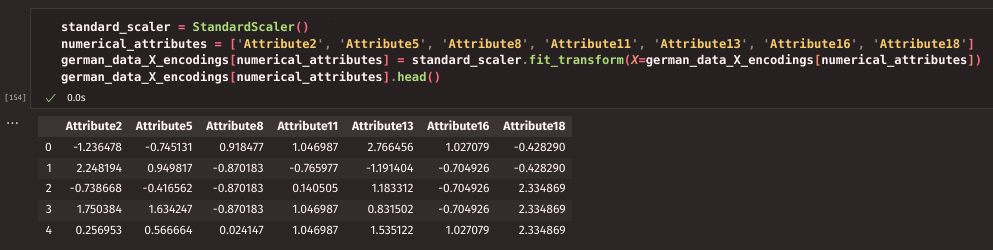
\includegraphics[width=\textwidth, height=0.2\textheight]{./I_1_g_i.png}
        \caption{[Standardized Numerical Features]}
    \end{figure}

    \subsection*{German Credit Data (Decision Tree)}

    SciKit-Learn's decision tree classifier requires non-string feature values. As such, we apply label encoding to all qualitative features in the German Credit dataset.
    \begin{figure}[H]
        \centering
        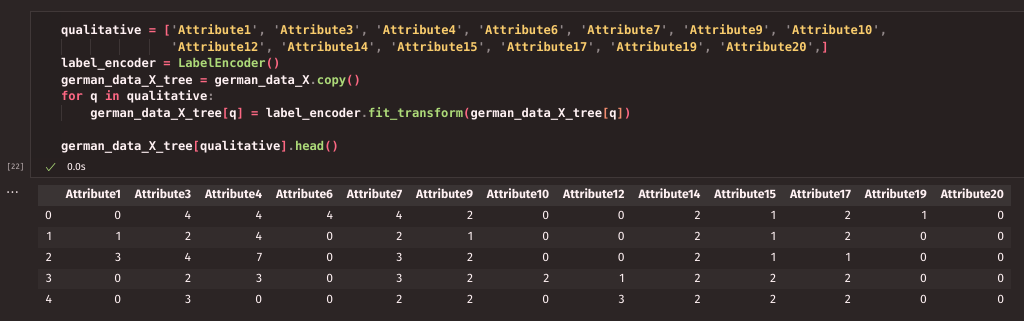
\includegraphics[width=0.9\textwidth, height=0.2\textheight]{./I_1_g_j.png}
        \caption{[Label Encoding German Data for Decision Tree Classification]}
    \end{figure}

    \subsection*{Waveform Data}

    All features of the waveform dataset are numeric by default with very similar scales making this dataset highly suitable for k-NN classification. The numeric data types
    are also compatible with scikit-learn's decision tree classifier. Hence, no preprocessing is required.

    \section*{Part I (Inference Efficiency):}

    \subsection*{K-NN (k=5) and Decision Tree (Greedy, GINI, No Max Depth)}

    \begin{figure}[H]
        \centering
        \begin{minipage}[t]{0.48\textwidth}
            \centering
            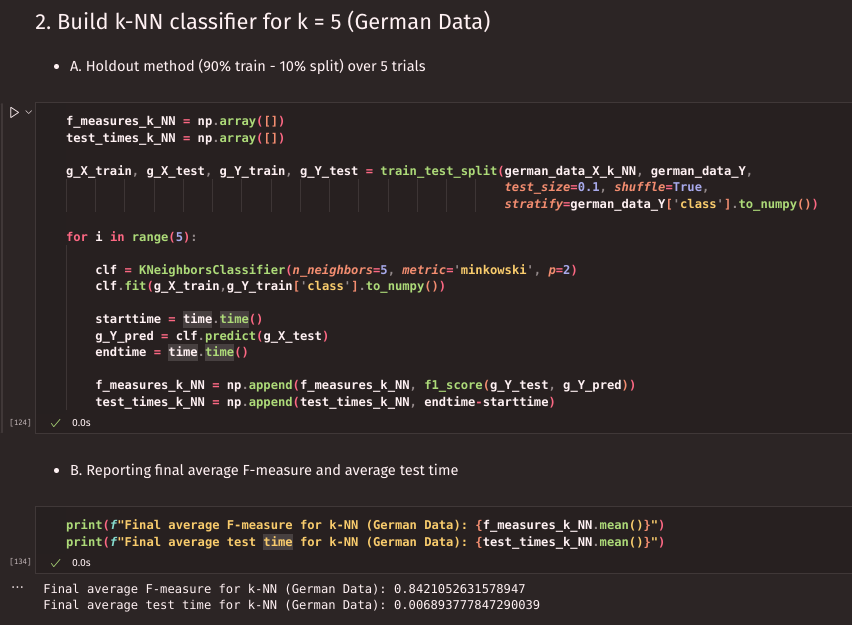
\includegraphics[width=\textwidth, height=0.25\textheight]{./I_2_g_a.png}
            \caption{[K-NN Classification for German Dataset]}
        \end{minipage}
        \hfill
        \begin{minipage}[t]{0.48\textwidth}
            \centering
            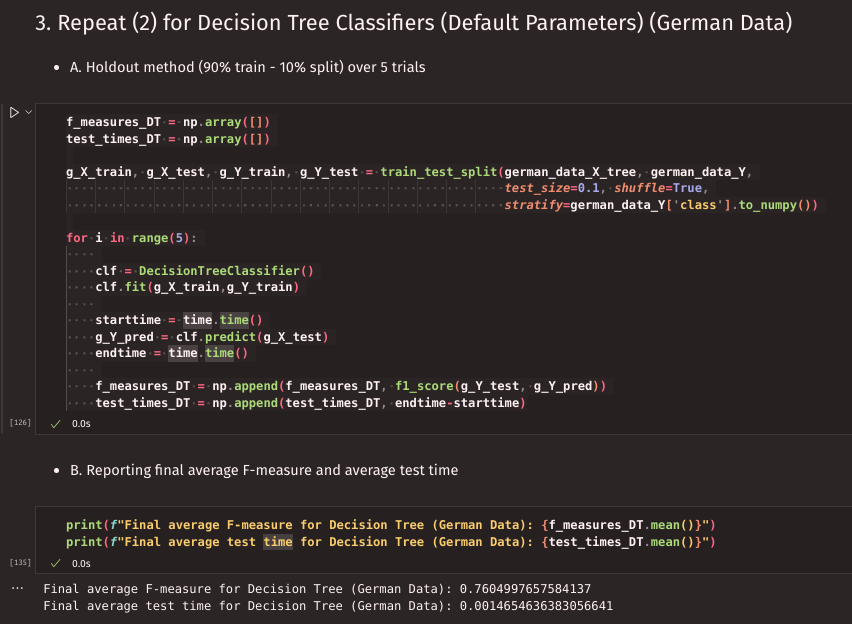
\includegraphics[width=\textwidth, height=0.25\textheight]{./I_2_g_b.png}
            \caption{[Decision Tree Classification for German Dataset]}
        \end{minipage}
    \end{figure}

    \begin{figure}[H]
        \centering
        \begin{minipage}[t]{0.48\textwidth}
            \centering
            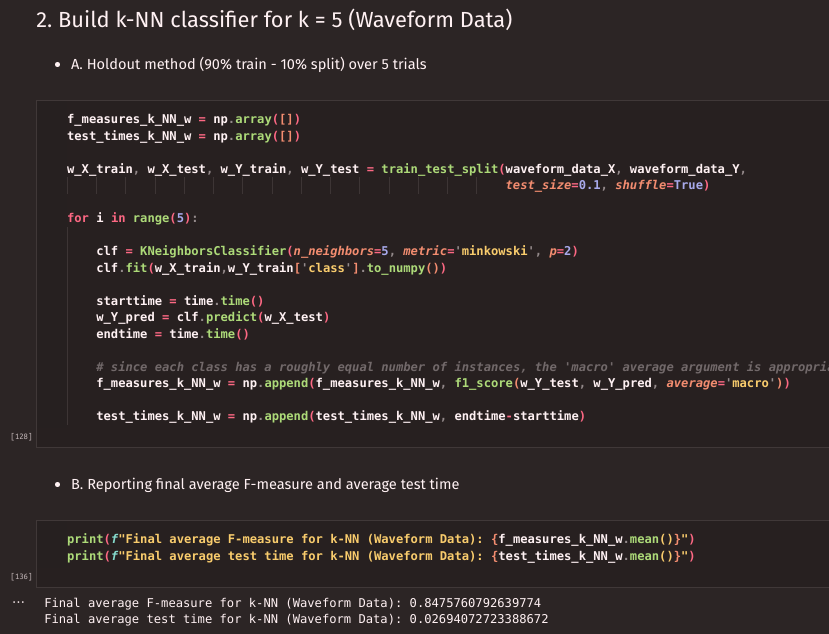
\includegraphics[width=\textwidth, height=0.25\textheight]{./I_2_w_a.png}
            \caption{[K-NN Classification for Waveform Dataset]}
        \end{minipage}
        \hfill
        \begin{minipage}[t]{0.48\textwidth}
            \centering
            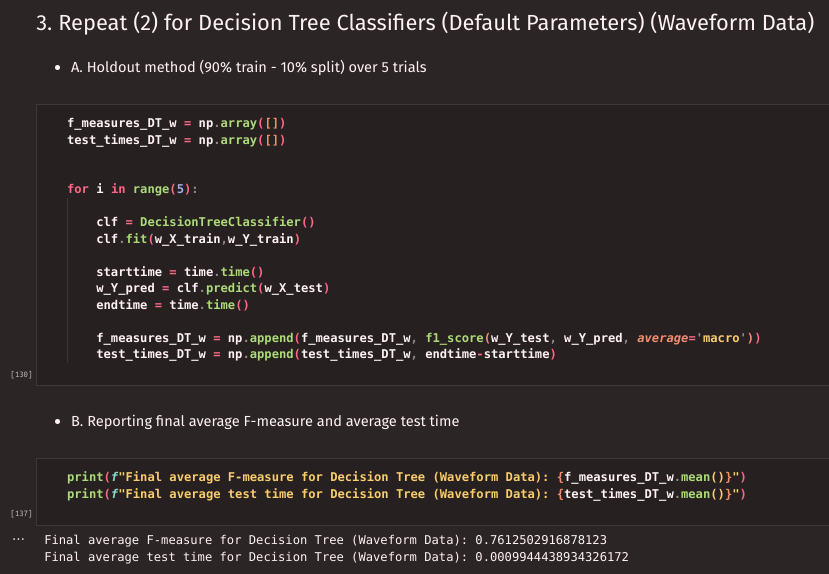
\includegraphics[width=\textwidth, height=0.25\textheight]{./I_2_w_b.png}
            \caption{[Decision Tree Classification for Waveform Dataset]}
        \end{minipage}
    \end{figure}

    \newpage

    \subsection*{Comparing Results}

    \begin{figure}[H]
        \centering
        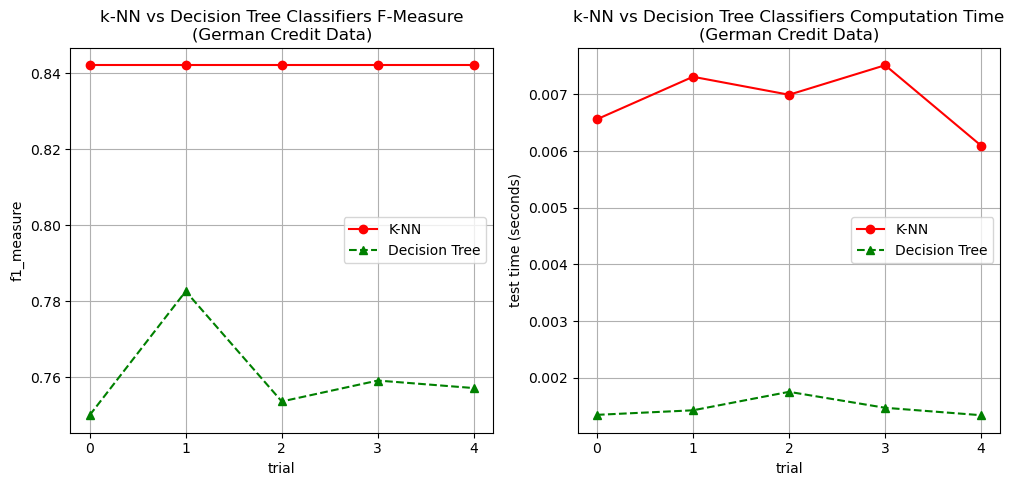
\includegraphics[width=0.9\textwidth, height=0.25\textheight]{./I_3_g.png}
        \caption{[K-NN vs Decision Tree Performance (German Dataset)]}
    \end{figure}
    \begin{figure}[H]
        \centering
        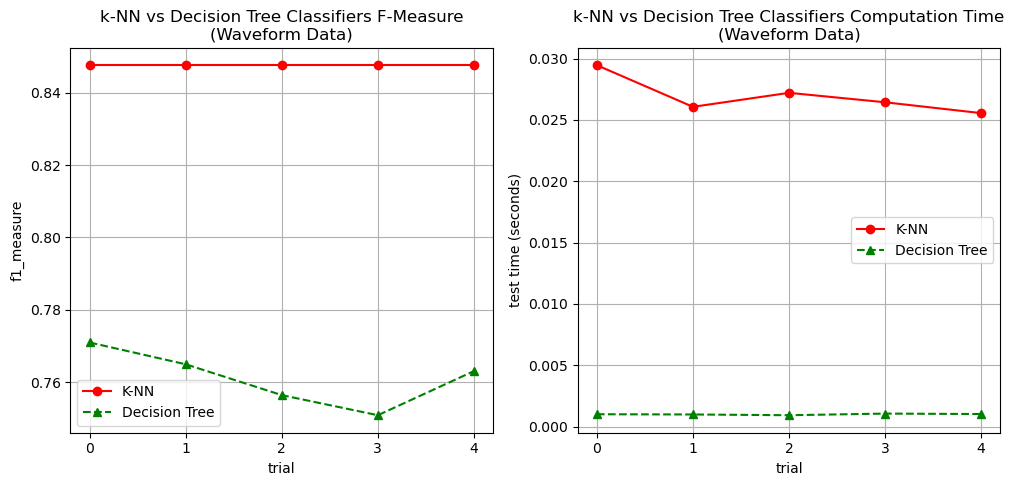
\includegraphics[width=0.9\textwidth, height=0.25\textheight]{./I_3_w.png}
        \caption{[K-NN vs Decision Tree Performance (Waveform Dataset)]}
    \end{figure}

    We see that k-NN is generally a more accurate form of classification than
    decision trees but also requires more elaborate preprocessing and greater
    inference times.
    
    \newpage

    \section*{Part II: Model Selection}
    \begin{figure}[H]
        \centering
        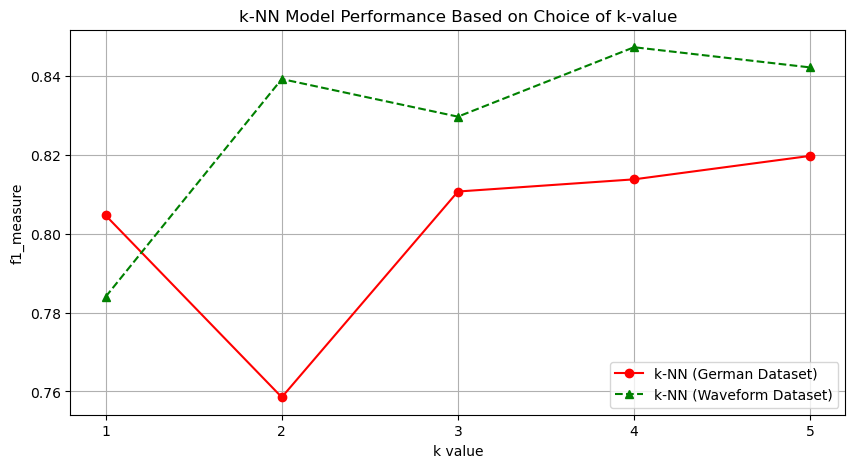
\includegraphics[width=0.9\textwidth, height=0.35\textheight]{./II_2.png}
        \caption{[K-NN Classification on Waveform and German Datasets for Different k]}
    \end{figure}

    Based on evaluations performed on the validation sets, the best k value for
    classifying Waveform data instances is k=4 and the best k value for classifying
    German credit data instances is k=5.

    \begin{figure}[H]
        \centering
        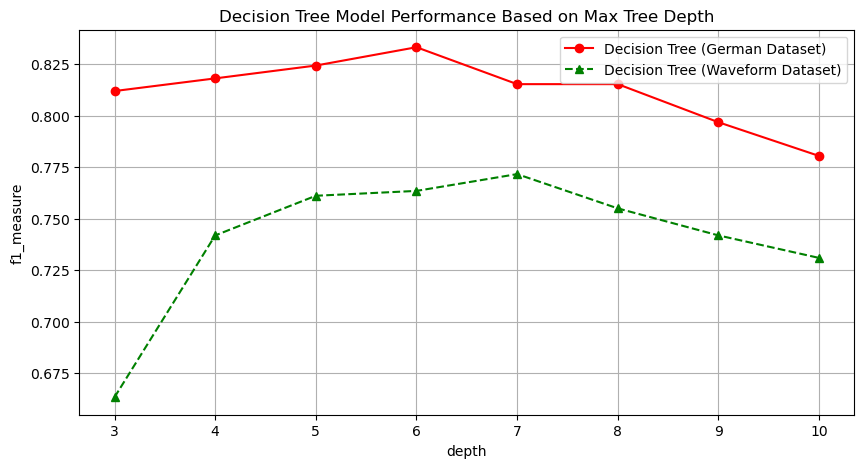
\includegraphics[width=0.9\textwidth, height=0.35\textheight]{./II_3.png}
        \caption{[Decision Tree Classification on Waveform and German Datasets with Different Max Depths]}
    \end{figure}

    Based on evaluations performed on the validation sets, the best max depth for
    classifying Waveform data instances is 7 and the best max depth for classifying
    German credit data instances is 6.

\end{document}